\chapter{Per-Frame Optimization}
\label{chap:per_frame}
The output of a DVS is a stream of events $\{e_k\}$, with
$e_k=\{x_k,y_k,t_k,p_k\}$ denoting its pixel coordinate, timestamp and
polarity, respectively. \Cref{fig:stream} shows the DVS output
interleaved with the APS output. We can clear see that the events are
triggered at the shape boundaries: when the sensor (or the scene) is
moving, these pixel locations will receive intensity changes. Thus DVS
works naturally as an edge detector.

\begin{figure}[h]
  \centering 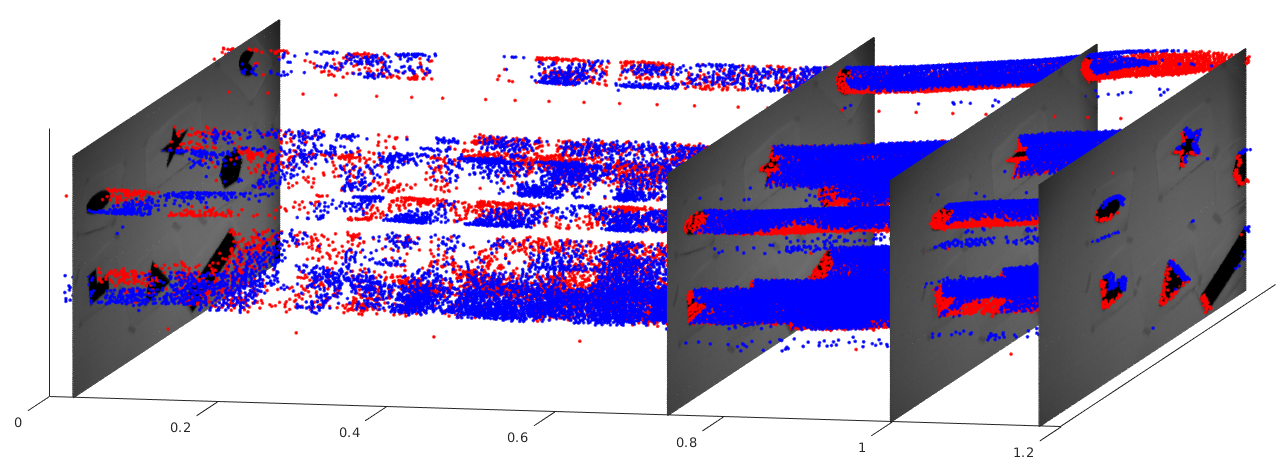
\includegraphics[width = \textwidth]{images/stream.png}
  \caption{Event stream plus grayscale images. During this period
    \num{100000} events and \num{27} frames are produced. Red and blue
    points denote the positive and negative events, respectively. DVS
    has a much higher output rate and is free from motion blur.}
  \label{fig:stream}
\end{figure}
Note that events can be triggered either by scene or camera motion. In
this work we assume a static scene and a moving camera.
\section{From Events to Frame}
\label{sec:event_warp}
A single event does not give much information. If we aggregate all the
events within a temporal window, depending on the size of the window
we may get different results as in \cref{fig:window_size_3}.

\begin{figure}[h]
  \begin{minipage}[t]{0.3\textwidth}
    \centering 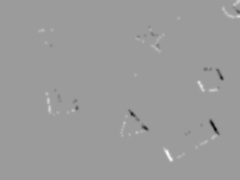
\includegraphics[width = \textwidth]{images/300.jpg}
    (a) \num{300}
  \end{minipage}
  \hfill
  \begin{minipage}[t]{0.3\textwidth}
    \centering 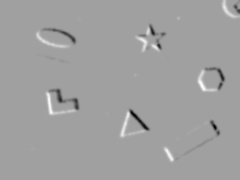
\includegraphics[width = \textwidth]{images/3000.jpg}
    (b) \num{3000}
  \end{minipage}
  \hfill
  \begin{minipage}[t]{0.3\textwidth}
    \centering 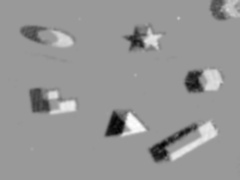
\includegraphics[width = \textwidth]{images/30000.jpg}
    (c) \num{30000}
  \end{minipage}
  \caption{The image generated by aggeragating \num{300}, \num{3000}
    and \num{30000} events. White and black dots represent positive
    and negative events, respectively. Gray indicates that no event is
    present in this pixel, or positive and negative events cancel each
    other out.}
  \label{fig:window_size_3}
\end{figure}
More specifically, we group a set of events
$\mathscr{E}\doteq \{e_k\}_{k=1}^N$ within a certain temporal window,
and synthesize an image by summing up the events. If we simply sum
along the time axis, the intensity at each pixel will be the sum of
the polarities of all the events that are triggered at this pixel
location within the window
\begin{equation}
  \label{eq:intensity}
  \mathcal{I}(\vec{x}) = \sum_{k=1}^N\pm_k\delta(\vec{x}-\vec{x}_k),
\end{equation}
with $\pm_k$ and $\vec{x}_k$ denoting the polarity and pixel
coordinates of the $k$th event, respectively. We call such synthesized
results in \cref{fig:window_size_3} as \emph{frames}.

The temporal resolution of a DVS in \citep{brandli2014240} is
\SI{1}{\micro s}; each event has a distinct timestamp, which also
indicates that events happen at distinct camera poses. Instead of
simply summing up events from different timestamps, a better strategy
is to project the events along the motion path, which is clearly
visible in \cref{fig:stream}, thus faithfully recover the scene edges
at a given time.

But how do we compute the motion path? Without additional motion
capture devices, we have no access to the ground truth pose; it's also
impossible to know the camera pose associated with each event, which
happens at such a high rate. To simplify the problem, we assume that
the camera moves at a constant velocity within an interval, which is
not a bad assumption if this interval is small enough. This group of
events are warped by the same model
$\vec{x}'_k=\mat{W}(\vec{x}_k,t_k;\theta)$, and the $\vec{x}_k$ in the
intensity computation \cref{eq:intensity} is substitute by
$\vec{x}'_k$. We find the optimal parameters $\theta$ that best
describes the events within this window, then shift the window to the
next set of events, and repeat this process.

There are several strategies available on choosing the window size. We
may group events by
\begin{enumerate}
\item a fixed time interval $\Delta t$,\\
\item a fixed number of events $N$ per subset,\\
\item dynamically adjusting the window size according to the current
  velocity.
\end{enumerate}
The first strategy is used in \citep{maqueda2018event}, they also
gives the comparison on different choice of window sizes. This might
be a good strategy when the motion estimation is needed at a fixed
rate. However, it suffers from the same problem as the traditional
camera, that is, it keeps producing redundant frames when no motion is
present. Also, a fixed time interval can not well compromise between
slow motion and rapid motion. Event cameras are data-driven cameras,
the output depends on the motion and the scene complexity, thus the
other two strategies are more favorable. \citep{zhu2017event} uses the
\emph{lifetime}\citep{mueggler2015lifetime} of the event to define the
window size, which depends on the event's velocity on the image
plane. Since the datasets we tested on each observes a same scene, the
scene complexity also stays almost the same within a certain
sequence. Thus we opt for the second strategy, and manually choose the
window size for each sequence.
% when the camera stops moving, no events will be generated, the pose
% will also not be further updated.

\section{Measuring the Sharpness of an Image}
\label{sec:contrast}
There are several metrics one could choose from to measure how well a
warp $\mat{W}$ is. Intuitively, the image would appear sharp if the
events are warped along its trajectory, otherwise motion-blurred.

the contrast of an image. A local contrast metric could be, for
example, convoluting the image with a high pass filter
\begin{equation}
  \label{eq:high_pass_filter}
  \mathcal{C}_H=
  \begin{bmatrix}
    -1&-1&-1\\
    -1&8&-1\\
    -1&-1&-1
  \end{bmatrix},
\end{equation}
and sum the pixel value of the filtered image. However, this metric
only compare a pixel with its 8 neighbors, thus an image with
scattered events (large noise) is also a valid configuration, as shown
in \cref{fig:contrast}(a). The Michelson contrast
\citep{michelson1995studies}, defined as
$\mathcal{C}_M=\left(\mathcal{I}_{\mathrm{max}}-\mathcal{I}_{\mathrm{min}}\right)/\left(\mathcal{I}_{\mathrm{max}}+\mathcal{I}_{\mathrm{min}}\right)$,
only considers the highest and lowest luminance in the image and is
thus more suitable to quantify contrast for periodic functions.

We choose to measure the contrast by the variance of the image,
defined by

\begin{equation}
  \label{eq:variance}
  \mathrm{Var}\left(\mathcal{I}\left(\vec{x};\bm{\theta}\right)\right)\doteq\frac{1}{\mid\Omega\mid}\int_{\Omega}\left(\mathcal{I}\left(\vec{x};\bm{\theta}\right)-\mu\left(\mathcal{I}\left(\vec{x};\bm{\theta}\right)\right)\right)^2d\vec{x},
\end{equation}
where $\mu\left(\mathcal{I}\left(\vec{x};\bm{\theta}\right)\right)$ is
the average image intensity. If the scene has more or less balanced
positive and negative events, the average will be close to
zero. Actually, since we only want to distinguish the edges with the
larger blank background, which indeed has zero intensity, we can also
simply substitute
$\mu\left(\mathcal{I}\left(\vec{x};\bm{\theta}\right)\right)$ with 0.

The goal of measuring the contrast of an image is to find the
configuration that aligns events triggered from the same visual
stimuli; thus the variance \cref{eq:variance} would be a very suitable
metric, as a squared metric favors the configuration that projects as
many events as possible to the same pixel.

Intergral sum pixels

\begin{figure}
  \begin{minipage}[t]{0.48\textwidth}
    \centering 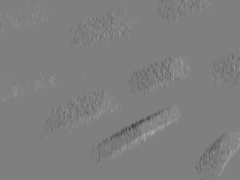
\includegraphics[width =
    \textwidth]{images/high_pass_contrast.png}
    % \label{subfig:texture}
    (a) An optimized frame using sharpening filter metric
  \end{minipage}
  \hfill
  \begin{minipage}[t]{0.48\textwidth}
    \centering 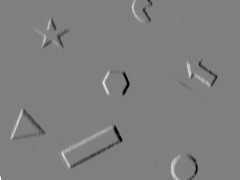
\includegraphics[width =
    \textwidth]{images/variance_contrast.png}
    % \label{subfig:map}
    (b) An optimized frame using variance metric
  \end{minipage}
  \caption{Comparison between two different metrics}
  \label{fig:contrast}
\end{figure}




\chapter{6DoF Pose Tracking in Planar Scenes}
\label{chap:planar_scenes}

Throughout this work the following notation is employed: $W$ denotes
the world frame, $C_1$ or $C_2$ denotes a camera frame.  $T_{AB}$ is
the transformation from frame $A$ to frame $B$, measured in frame $A$.

$\vec{X}$ the position of the event with respect to world or camera
frame, $\vec{x}$ the calibrated coordinates of the event.


\subsection{Planar Homography}

\label{sec:planar_homo}
The warp function $\vec{x}'=\mat{W}(\vec{x},t;\bm{\theta})$ does not only
depend on the motion parameters, but also the scene parameters, which
is the unknown depth.  In the case of a planar scene the problems
simplifies, since a plane $\mathbf{P}$ can be parameterized by two
sets of parameters: $\vec{n}\in\mathbb{S}^2$ the unit surface normal
of $\mathbf{P}$ with respect to the current camera frame, and $d$ the
distance from the camera center to $\mathbf{P}$. The warp function
then becomes
\begin{align}
  \vec{X}'=&\mat{R}(t)\vec{X}+\vec{T}(t)\\
  \vec{X}=&\mat{R}(t)^\top\left(\vec{X}'-\vec{T}(t)\right)\\
  \vec{X}=&\mat{R}(t)^\top\left(\mat{I}+\vec{T}(t)\vec{n}^\top/d\right)\vec{X}',  \label{eq:planar_homo_0}
\end{align}
thus
$\vec{x}'\sim\left(\mat{R}(t)^\top\left(\mat{I}+\vec{T}(t)\vec{n}^\top/d\right)\right)^{-1}\vec{x}$.
Here $(\mat{R}(t), \vec{T}(t))\in SE(3)$ denotes the relative pose
between two cameras at which the current event being warped and the
first event within the window happened, and $t$ is the relative
timestamp with respect to the first event. Under a constant velocity
model with linear velocity $\vec{v}\in\mathbb{R}^3$ and angular
velocity $\bm{\omega}\in\mathbb{R}^3$, the translation is given by
\begin{equation}
  \label{eq:translation}
  \vec{T}(t)=\vec{v}t,
\end{equation}
the rotation matrix is given by the \textit{exponential map} exp:
$\mathfrak{so}(3)\rightarrow SO(3)$:
\begin{equation}
  \label{eq:rotation}
  \mat{R}(t)=\mathrm{exp}(\bm{\omega}^\wedge t),
\end{equation}
where $^\wedge$ is the \textit{hat} operator
\begin{equation}
  \label{eq:hat}
  \bm{\omega}^\wedge=
  \begin{bmatrix}
    \omega_1\\\omega_2\\\omega_3
  \end{bmatrix}
  =
  \begin{bmatrix}
    0&-\omega_3&\omega_2\\
    \omega_3&0&-\omega_1\\
    -\omega_2&\omega_1&0
  \end{bmatrix}
  \in\mathfrak{so}(3).
\end{equation}

\section{From Frames to Map}
\label{sec:frame2map}
The contrast maximization procedure in the above section optimizes the
relative pose between successive frames. We show in this section that
the same idea can be applied to perform global pose tracking in planar
scenes. We first explain how the map is defined, and how to track a
known map, then we shown how this map is built by selecting a set of
keyframes.

\subsection{Map}
\label{sec:map}
A map is a plane with three components: the normal direction
$\vec{n}_w$, the distance $d_w$ to the origin, and the texture; the
texture of a map represents all the edges on the plane. \Cref{fig:map}
shows the an example of such map. \Cref{fig:map}(a) also shows the set
of keyframes used to construct the map. We will talk more about
keyframes in \cref{sec:keyframe2map}. The global coordinate is chosen
as the camera coordinate of the first frame.

\begin{figure}
  \begin{minipage}[t]{0.48\textwidth}
    \centering 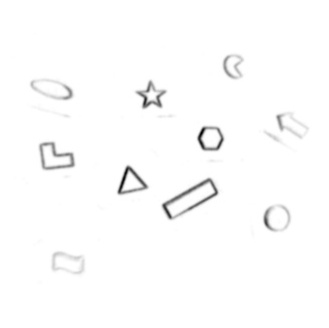
\includegraphics[width =
    \textwidth]{images/map_805.jpg}
    % \label{subfig:texture}
    (a) The texture of a map
  \end{minipage}
  \hfill
  \begin{minipage}[t]{0.48\textwidth}
    \centering 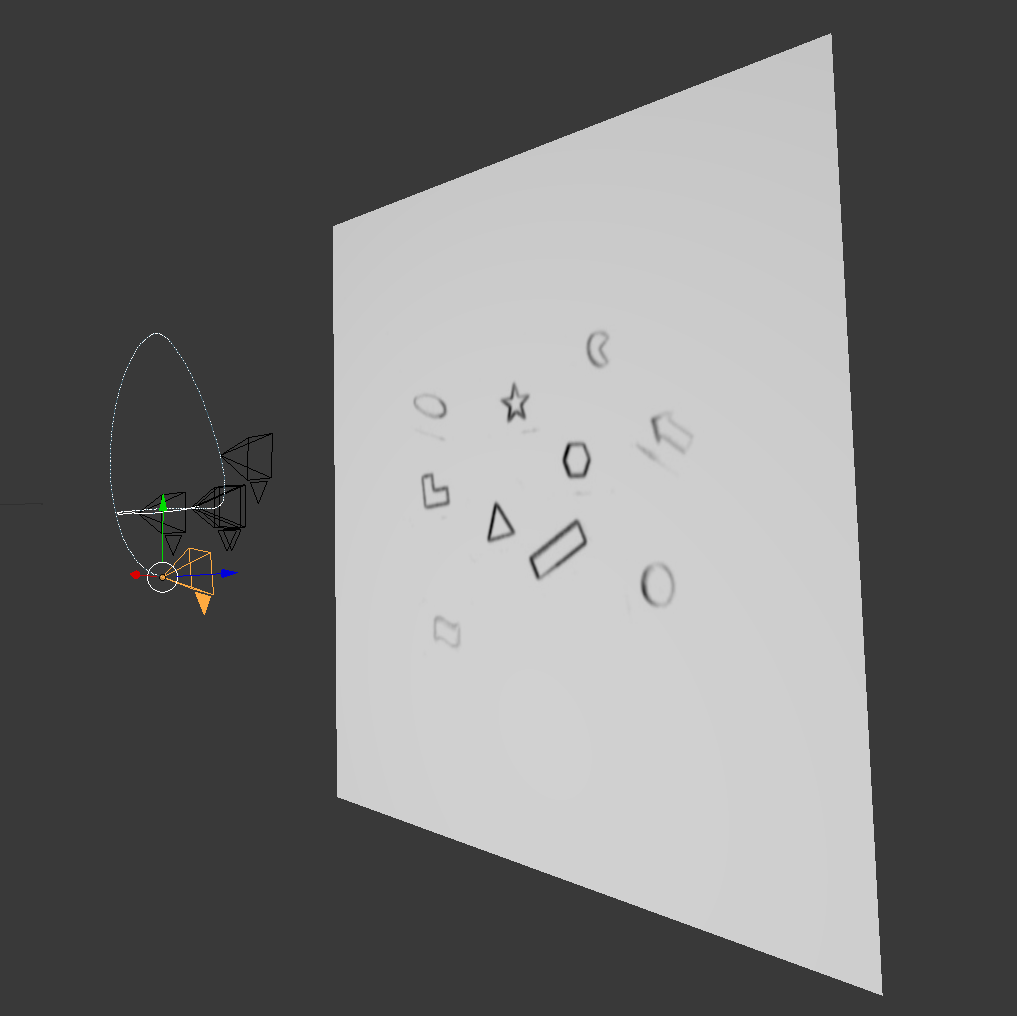
\includegraphics[width = \textwidth]{images/4.png}
    % \label{subfig:map}
    (b) A map in the global frame
  \end{minipage}
  \caption{Map}
  \label{fig:map}
\end{figure}



\subsection{Tracking}
\label{sec:tracking}
Suppose a map is present, then the normal direction $\vec{n}_w$ of the
plane and the distance $d_w$ to the origin are known. Also the pose of
the current frame $(\mat{R}_{wc}, \vec{T}_{wc})\in SE(3)$ is
determined by the motion estimation from the last frame (a quick note
to the terminology we are using: whenever we say the \textit{pose} of
a frame, we always refer to the camera \textit{pose} at which the
first event within the frame happens). The parameters left to be
estimated for each frame is
$\phi=\left(\bm{\omega},\vec{v}\right)\in\mathbb{R}^6$. By
substituting $\vec{n}$ with $\vec{n}_c = \mat{R}_{cw}\vec{n}_w$, and
$d$ with $d_c = d_w+\vec{T}_{wc}\cdot\vec{n}_w$ in
\cref{eq:planar_homo_0}, we get the homography matrix within each
frame as
\begin{equation}
  \label{eq:planar_homo_1}
  \mat{H}_1=\mat{R}^\top\left(\mat{I}+\vec{T}\vec{n}_c^\top/d_c\right)
\end{equation}
and $\vec{x}'_c\sim\mat{H}_1^{-1}x_c$.

A nonlinear optimizing problem naturally suffers from local
optima. Without a good initialization, the motion computed with the
method in \cref{sec:event_warp} could sometimes be a local optimum
delivering an image that appears sharp, despite being wrongly
estimated (see \cref{fig:local_optimum}). In order to make sure that
the estimated motion from the per frame contrast maximization also
conform to the global map. Thus we perform another optimization, where
we project the events of the current frame to the global map. The
parameter set is still $\left(\bm{\omega}^\top,\vec{v}^\top\right)$,
and we use the output from last procedure as an initial guess.

The procedure described in the first paragraph of this section can be
understood as projecting the events on a \textit{blank
  canvas}. Similarly, in the projecting-to-map procedure we project
the events on the \textit{texture} of the map, and measure the
strength of the synthesized image with the same variance function as
in \cref{eq:variance}, thus finding the set of the parameters that
best align the events in the current frame to their correspondences in
the texture.

The projection from an event to the map is
\begin{equation}
  \label{eq:frame2map}
  \vec{x}_w \sim \mat{R}_n\mat{H}_2^{-1}\mat{H}_1^{-1}\vec{x}_c,
\end{equation}
with $\mat{R}_n$ the transformation from the orientation of the global
frame to the orientation of the map, computed by
\begin{align}
  \mat{K}& =(\vec{n}_w\times \vec{z})^\wedge\\
  \mat{R}_n&=\mat{I} +\mat{K} + \mat{K}^2/ (1 +  \vec{n_w}\cdot\vec{z}),  \label{eq:global2map}
\end{align}
where $\vec{z}=(0,0,-1)$ denotes the plane fronto-parallel to the
camera, and
\begin{equation}
  \label{eq:frame2global}
  \mat{H}_2 = \mat{R}_{cw}\left(\mat{I} + \vec{T}_{wc}\vec{n}^\top/d_w\right)
\end{equation}
is the projection from the current frame to the global frame, with
$\mat{R}_{wc}, \mat{T}_{wc}$ being the pose of the current
frame. $\mat{H}_1$ is the planar homography for each frame as in
\cref{eq:planar_homo_1}. But the $\mat{R}(t)$ and $\vec{T}(t)$ might
be different since we are refining these parameters.

After projecting, we obtain an image composed of the map texture and
the events of the current frame. We maximize the contrast of this
image using the cost function defined in \cref{eq:variance}. The
optimized velocity is used for propagating the pose to the next
incoming frame via
\begin{align}
  \label{eq:pose_propagation}
  \vec{T}_{wc_2}&=\mat{R}_{wc_1}\vec{v}\Delta t+ \vec{T}_{wc_1}\\
  \mat{R}_{wc_2}& =\mat{R}_{wc_1}\mathrm{exp}(\bm{\omega}^\wedge \Delta t),
\end{align}
where $c_1$ and $c_2$ denotes the current frame and the next frame,
respectively, and $\Delta t$ is the temporal size of the current
frame.

\begin{figure}
  \begin{minipage}[t]{0.48\textwidth}
    \centering 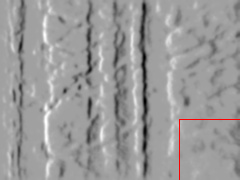
\includegraphics[width =
    \textwidth]{images/slider_estimation.png}
    \label{subfig:estimation}
    (a) Estimation
  \end{minipage}
  \hfill
  \begin{minipage}[t]{0.48\textwidth}
    \centering 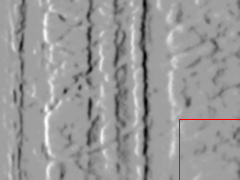
\includegraphics[width =
    \textwidth]{images/slider_groundtruth.png}
    \label{subfig:groundtruth}
    (b) Groundtruth
  \end{minipage}
  \hfill

  \begin{minipage}[t]{\textwidth}
    \centering 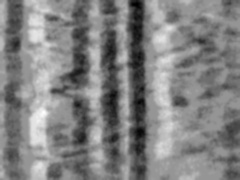
\includegraphics[width =
    0.48\textwidth]{images/slider_zero_motion.jpg}
    \label{subfig:estimation}
    \\(c) Without motion compensation
  \end{minipage}
  \hfill

  \caption{An example of local optima. This is the dataset
    \textit{slider\_hdr\_close} with a window size of 50000
    events. (a) shows the optimized image with \textit{linear
      velocity} $( 0.231, 0.109, 0.256)$, \textit{angular velocity}
    $(0.405, -0.130, -0.278)$ and \textit{plane normal}
    $(-0.579, 0.282, -0.765)$. (b) shows the result using groundtruth
    parameters with \textit{linear velocity} $(0.163, 0, 0)$,
    \textit{angular velocity} $(0, 0, 0)$ and \textit{plane normal}
    $(0, 0, -1)$. Both images appear mostly identical, though at the
    lower right corner, for example, one can still recognize the
    difference. Also both images look much sharper than the image
    without motion compensation in (c). It is worth mentioning that
    the contrast of the estimation is actually slightly larger than
    that of the groundtruth}
  \label{fig:local_optimum}
\end{figure}

\subsection{Mapping}
\label{sec:keyframe2map}

After having collected the first $N$ events, we start the mapping
process. For the first frame we estimate the full parameter set
$\phi=\left(\bm{\omega}^\top,\vec{v}^\top/d_w,\varphi,\psi\right)^\top\in\mathbb{R}^8$,
where $\left(\varphi, \psi\right)$ parametrize the unit vector of the
plane normal, and $\vec{v}^\top/d_w$ account for the scale ambiguity
problem introduced in linear velocity estimation from monocular
camera. We can for example determine the scale of the scene by setting
$d_w$ to $1m$, then scales of the consecutive frames are also
determined by $d_c = d_w+\vec{T}_{wc}\cdot\vec{n}_w$.

From the optimized first frame we initialize the map, by projecting
the frame to the planar scene via a rotation $\mat{R}_n$ as in
\cref{eq:global2map} \textcolor{red}{(you might have implemented this
  part wrong)}. Then we can track the next frames with this map using
the method described in \cref{sec:tracking}.

As the camera moves, there might be new information available in the
scene, so that the map needs to be expanded. After optimization for
each single frame, we also measure the \textit{per-pixel-overlap}
between the frame and the map,S that is, how many percent pixels in the
frame can be explained by the map. The overlap might be small, when
the camera is just exploring a new area so that only part of the frame
and the map is overlapping; another possibility is that the map is not
accurate enough to explain the current frame, which often happens when
only one frame is used until now to construct the map. When the
overlap reaches a certain threshold (0.8 for example), we try to
insert a new \textit{keyframe}.

When the system decides that a new keyframe is needed, we collect all
the keyframes until now, plus the current frame, which is a keyframe
candidate, and optimize the poses and velocities of these frames, as
well as the map together. Suppose there are $k$ frames (including the
keyframe candidate), the to be optimized parameter set is
\begin{equation*}
  \phi=\left(\mat{R}_{(1\sim k)},\vec{T}_{(1\sim
      k)},\bm{\omega}_{(0\sim k)},\vec{v}_{(0\sim
      k)}/d_w,\varphi,\psi\right)\in\mathbb{R}^{12k-4}.
\end{equation*}
Here $1\sim k$ means from frame $1$ to frame $k$, and we skip the pose
optimization of frame $0$, which is the first frame, since it defines
the global coordinate. We project all the events of these $k$ frames
to the plane parametrize by $(\varphi,\psi)$ with \cref{eq:frame2map},
and again optimize the contrast of the synthesized image the obtain
the optimal parameter set.

Note that in the mapping process we drop the polarity of the event,
since different keyframes might include events from the same visual
stimuli but triggered when moving in different directions, when summed
together the polarities might cancel each other out. For the same
reason, we also don't use the polarity when matching a frame to the
map.

After this step, we also measure the \textit{per-pixel-overlap}
between the keyframe candidate and the image synthesized by the other
keyframes, with the newly optimized parameter set. If this is a good
match \textcolor{red}{(define a good match)}, we continue the
tracking. Otherwise, we consider the pose estimation of the current
frame to be already off. In this case we preserve the former map, and
use this map to start the \textit{relocalization} procedure.

\subsection{Relocalization}
\label{sec:relocalization}

\section{Experiments}
\label{sec:experiments}
The algorithm is tested on four planar datasets provided by the
\textit{Robotics and Perception Group} at UZH
\citep{mueggler2017event}, which includes \textit{poster\_6dof,
  poster\_translation, shapes\_6dof, shapes\_translation}. The
\textit{shapes} dataset contains several simple shapes on the wall,
whereas the \textit{poster} contains richer rock texture. A planar
assumption is redundant for the rotation datasets and thus the results
are not listed for comparison here.

We define the camera axes as in \cref{fig:axes}. The camera coordinate
frame of the first synthesized frame is set as the global coordinate
frame. The x, y and z axes are also pitch yaw, roll axes,
respectively.

\begin{figure}
  \begin{minipage}[t]{0.48\textwidth}
    \centering 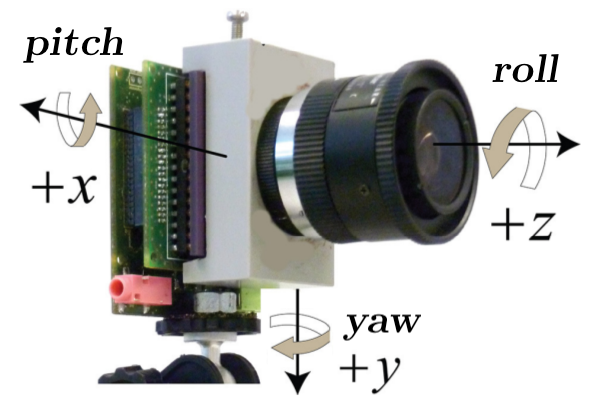
\includegraphics[width = \textwidth]{images/axes.png}
    (a)
  \end{minipage}
  \hfill
  \begin{minipage}[t]{0.48\textwidth}
    \centering 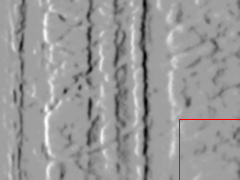
\includegraphics[width =
    \textwidth]{images/slider_groundtruth.png} (b)
  \end{minipage}
  \hfill
  \caption{Axes definition}
  \label{fig:axes}
\end{figure}
\Cref{fig:shapes_6dof_pose} shows the comparison of the results of the
proposed method against ground truth on the whole
\textit{shapes\_6dof} sequence. We observe that the orientation and
translation estimation along z axis is the most accurate among all the
axes; when zoomed in (\cref{fig:shapes_6dof_pose_zoomed}), it is clear
to see that the roll estimation is almost indistinguishable from the
ground truth. We split the quantitative error estimation for
orientation along 3 axes (\cref{tab:err_est}), in order to show that
this holds true for all the datasets we tested on. In these datasets,
the global z axis is close to the plane normal; we believe that the
events generated by a motion along the plane normal direction is more
obvious, and also harder to be explained by a combination of other
motions, and are thus more reliable.

We also observe in \cref{fig:shapes_6dof_pose} that in the latter half
of the sequence there are larger fluctuations. There are multiple
reasons for that:
\begin{enumerate}
\item The window size is not suitable

  The window size is manually chosen for each dataset. A range of
  $2000 - 5000$ usually works good for the \textit{shapes} datasets,
  since the scene consists of simple regular
  shapes. \Cref{fig:window_size}(a) shows what the camera frustum
  normally contains. However, in the rapid movement phase, the camera
  very often moved to a position where other scenes which don't belong
  to \textit{shapes} also becoms visible. \Cref{fig:window_size}(b)
  shows the scene of \textit{shapes\_6dof} at around 47.8 seconds. At
  this moment the poster on the wall is also visible, which actually
  belongs to the \textit{poster} sequences. The poster has much more
  complex textures, when performing pose estimation on the
  \textit{poster} sequences, we normally choose a window size of
  $30000-50000$. Apparently, a window size of 4000 is no longer enough
  in this case, which causes the motion estimation in this period
  being inaccurate.
  \begin{figure}
    \begin{minipage}[t]{0.48\textwidth}
      \centering 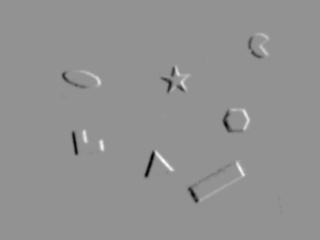
\includegraphics[width =
      \textwidth]{images/window_size_good.jpg} (a)
    \end{minipage}
    \hfill
    \begin{minipage}[t]{0.48\textwidth}
      \centering 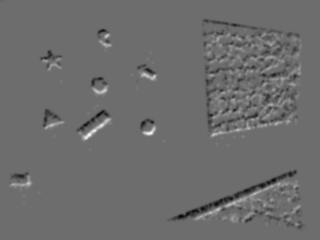
\includegraphics[width =
      \textwidth]{images/window_size_bad.png} (b)
    \end{minipage}
    \hfill
    \caption{A window size of $4000$ for a specific dataset
      \textit{shapes\_6dof} but different scene complexity}
    \label{fig:window_size}
  \end{figure}
\item There are few textures available

  A very representative example is that when tracking the dataset
  \textit{shapes\_translation}, we always get lost at around $23
  sec$. Investigating the scene around this time instance
  (\cref{fig:shapes_tr_lost}(a)), we found that very few or even no
  texture is available. It's also not possible to perform a reliable
  pose estimate during this period. For the \textit{per-frame}
  velocity estimation proposed in
  \citep{gallego2017accurate,gallego2018unifying}, where each frame is
  uncorrelated \textcolor{red}{?}, this is usually not a serious
  problem, since when the textures becomes available again, the
  optimization pipeline is still able to continue, it just might be
  harder to start from a bad initialization. However, for the pose
  estimation where a cumulative result is needed, a few bad estimated
  frames might destroy the whole following sequence.

  The \textit{bundle adjustment} and \textit{relocalization} parts of
  the pipeline is designed to deal with such situations. However, a
  bad initial guess of the pose $(\mat{R},\vec{T})$ is generally
  harder to start with than a bad initial guess of velocities
  $(\bm{\omega},\vec{v})$. When the pose estimation from last frame is
  already too off, after optimization there might still be little
  overlap between the current frame and the pose. This is when the
  \textit{bundle adjustment} tries to insert a keyframe and track from
  the new keyframe. The current implementation doesn't reinitialize
  the map after the tracking is lost. The advantage is that there is
  still chance to come back to the original map after tracking a wrong
  ``local map'' (\cref{fig:shapes_tr_lost}(b)); the disadvantage is
  that the global map will most likely be polluted by the ``local
  map'' (\cref{fig:shapes_tr_lost}(c))
  \begin{figure}
    \begin{minipage}[t]{0.48\textwidth}
      \centering 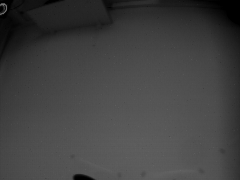
\includegraphics[width =
      \textwidth]{images/frame_00000520.png} (a) There is little
      texture visible
    \end{minipage}
    \hfill
    \begin{minipage}[t]{0.48\textwidth}
      \centering 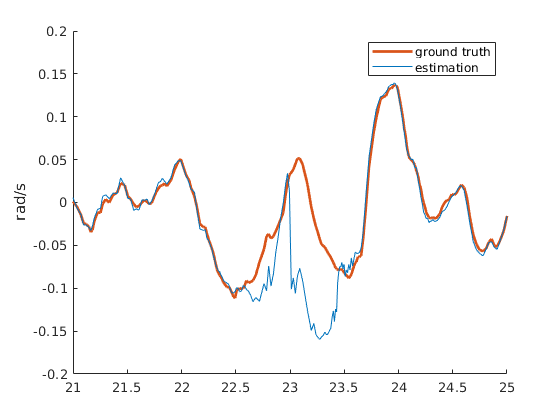
\includegraphics[width =
      \textwidth]{images/shapes_tr_lost.png} (b) Relocalized after get
      lost (roll component)
    \end{minipage}

   \begin{minipage}[t]{0.48\textwidth}
     \centering 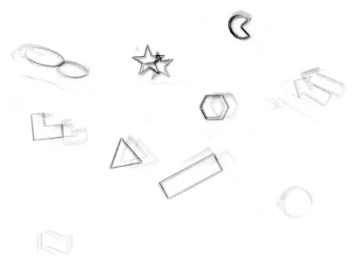
\includegraphics[width =
     \textwidth]{images/map_956.jpg} (c) Polluted map after tracking
     is lost
   \end{minipage} \caption{When tracking the dataset
     \textit{shapes\_translation}, we always get lost at around
     $23 sec$, but there is still chance to relocalize}
   \label{fig:shapes_tr_lost}
 \end{figure}

\end{enumerate}

\begin{figure}
  \begin{minipage}[t]{\textwidth}
    \centering 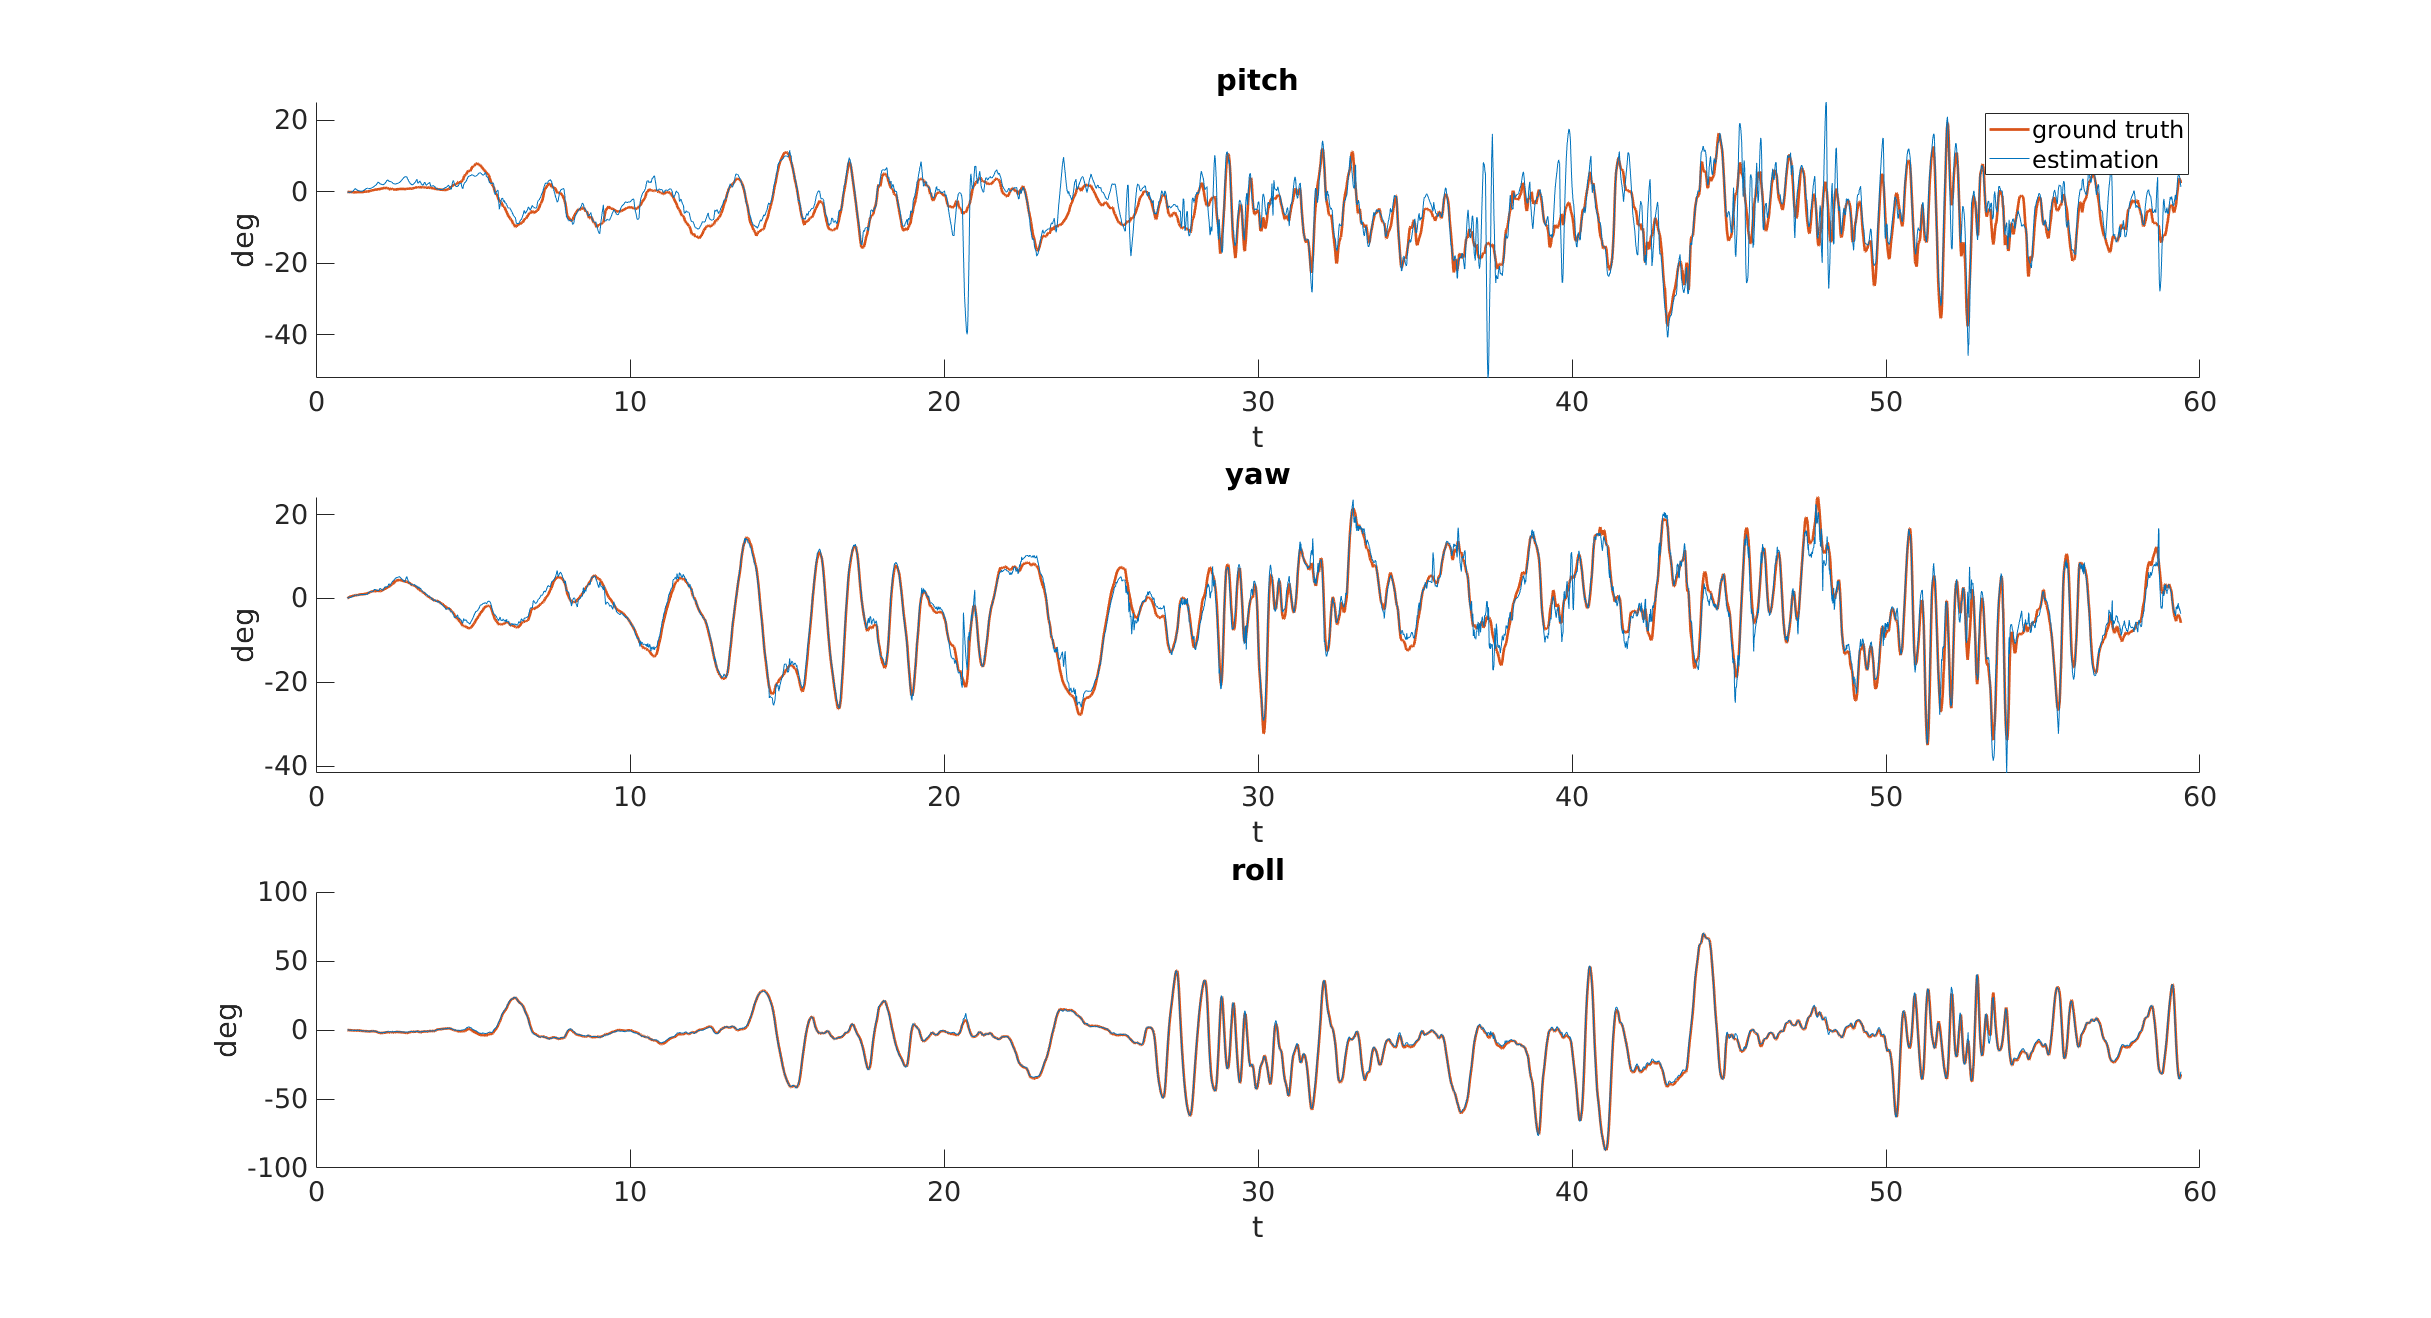
\includegraphics[trim={5cm 0cm 5cm 0cm},clip,width =
    \textwidth]{images/shapes_6dof_rotation.png} (a) Orientation
  \end{minipage}
  \hfill
  \begin{minipage}[t]{\textwidth}
    \centering 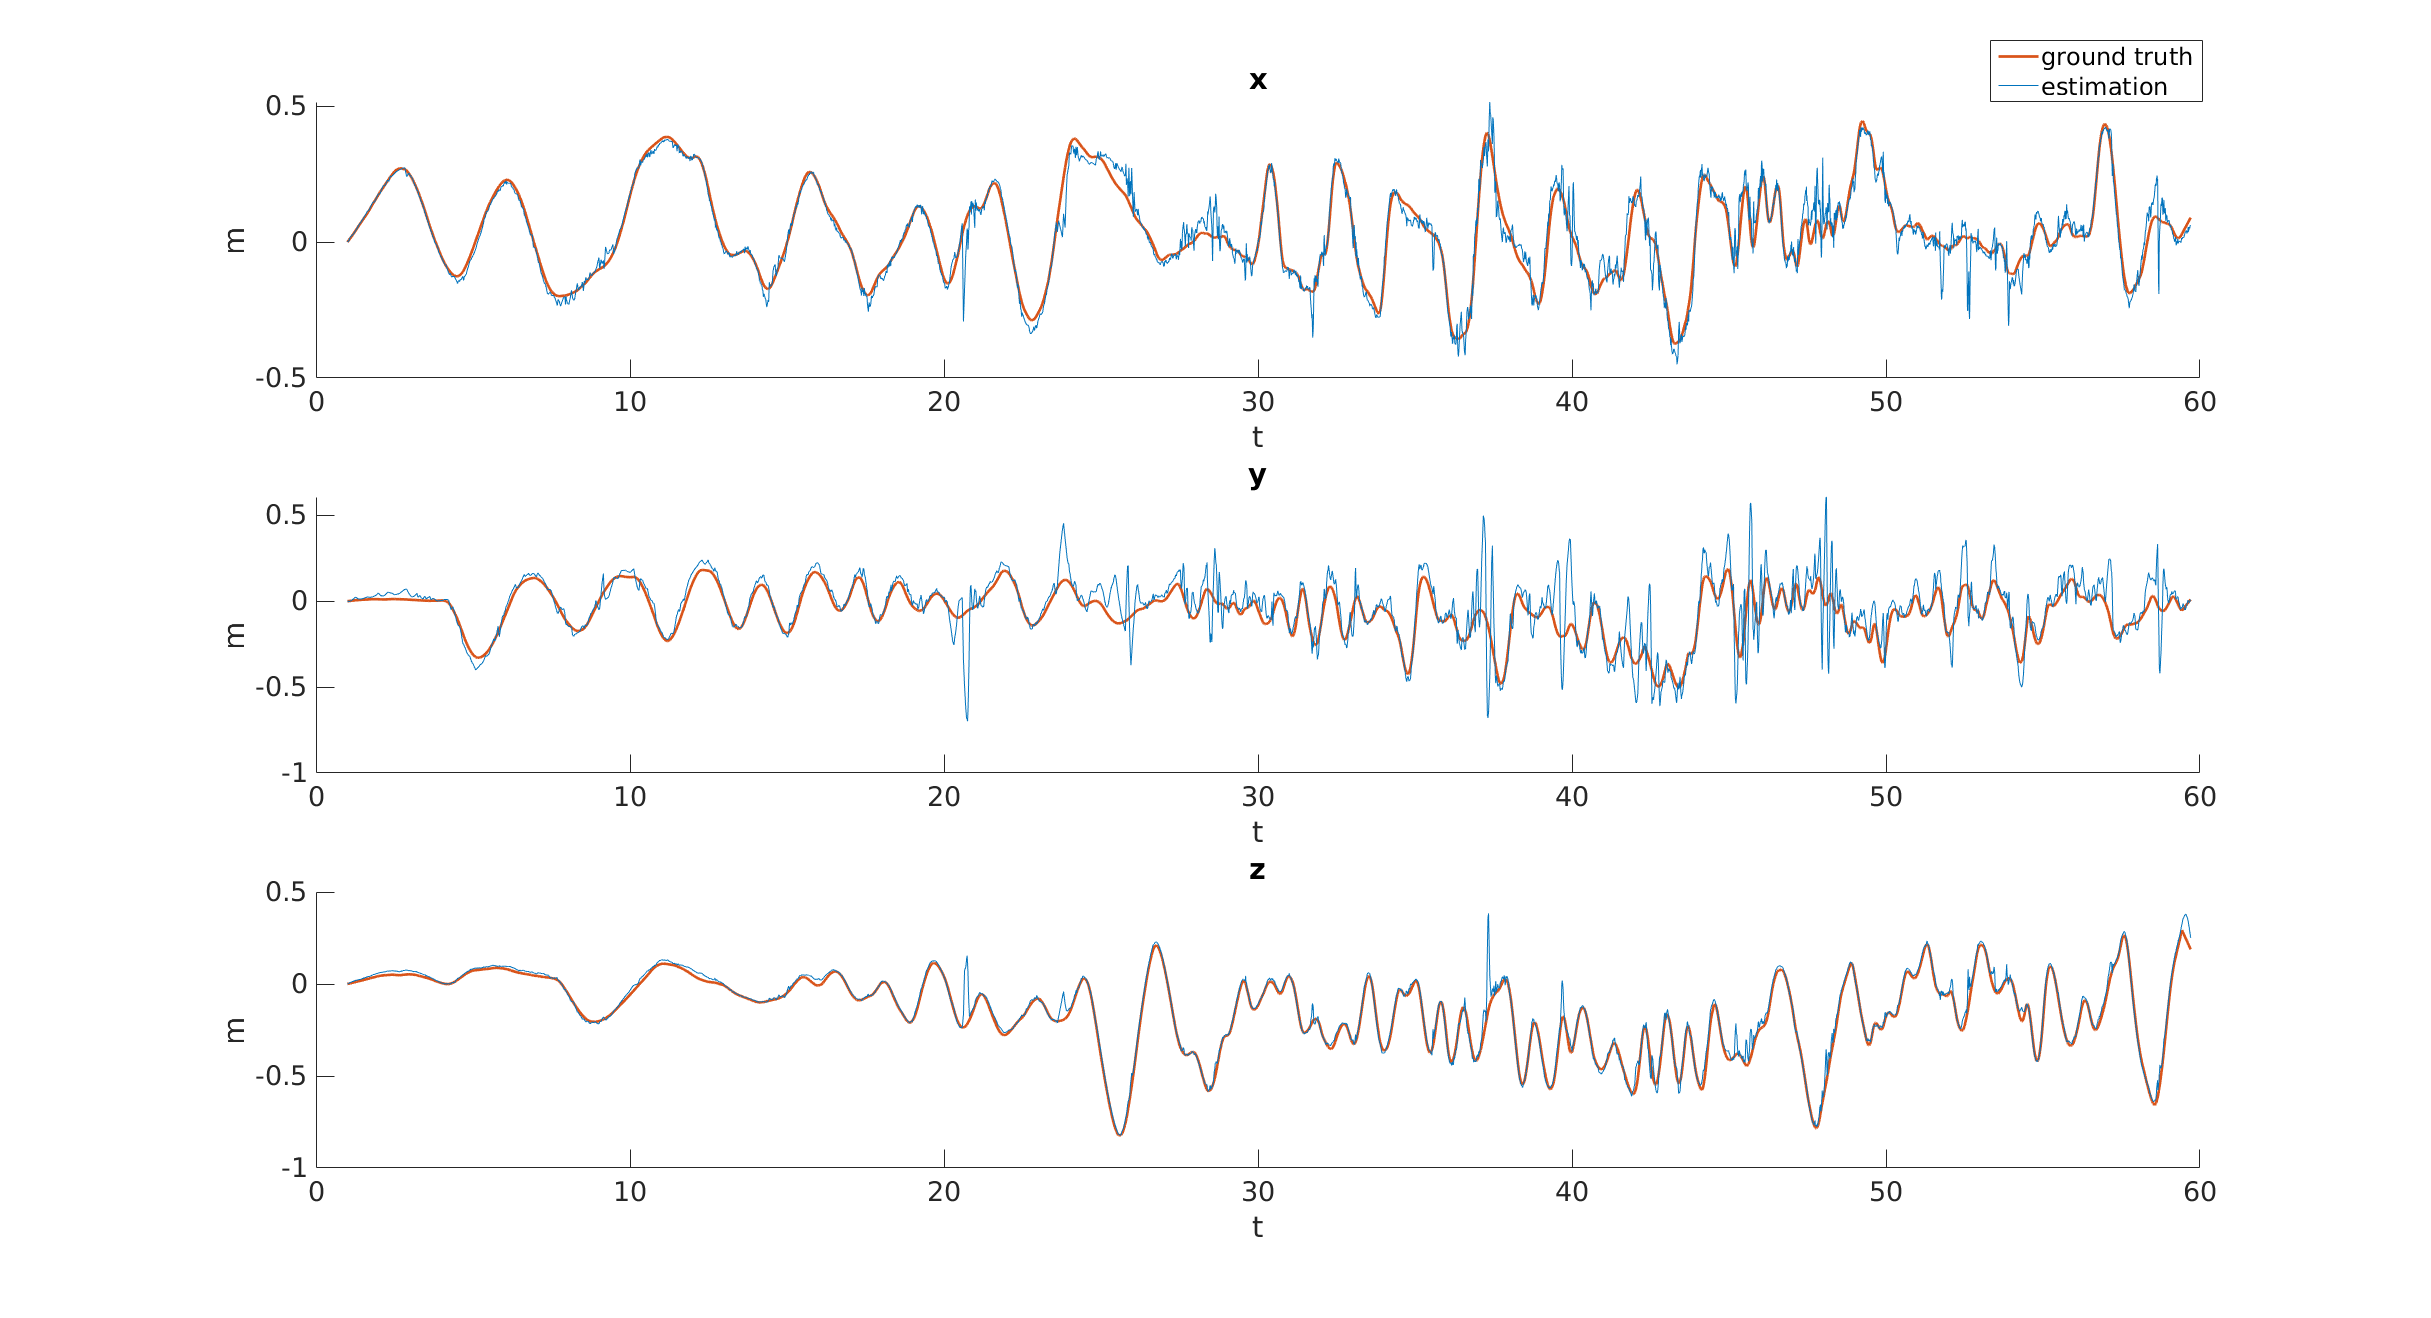
\includegraphics[trim={5cm 0cm 5cm 0cm},clip,width =
    \textwidth]{images/shapes_6dof_translation.png} (b) Translation
  \end{minipage}
  \hfill
  \caption{\textit{shapes\_6dof} sequence. Comparison of the estimated
    pose (blue line) against ground truth (red line).}
  \label{fig:shapes_6dof_pose}
\end{figure}

\begin{figure}
  \begin{minipage}[t]{0.48\textwidth}
    \centering 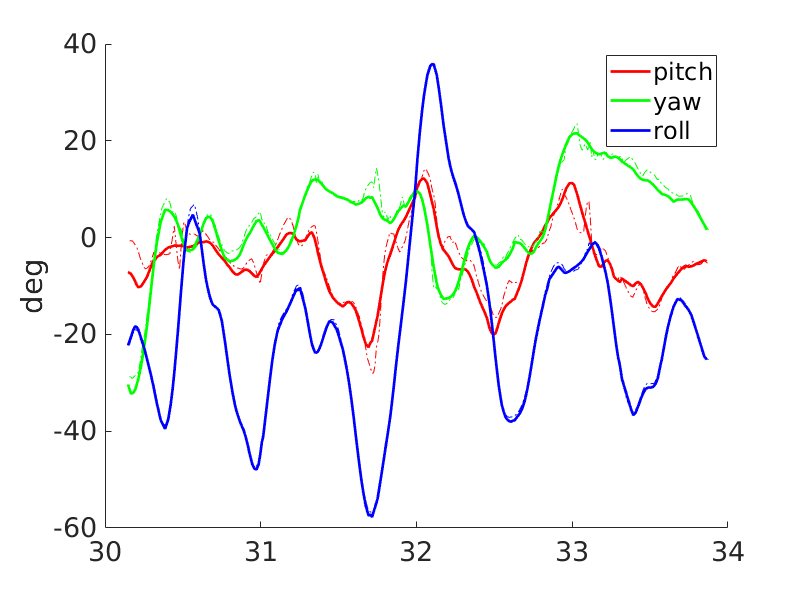
\includegraphics[width =
    \textwidth]{images/shapes_6dof_rotation_33.png} (a) Orientation
  \end{minipage}
  \hfill
  \begin{minipage}[t]{0.48\textwidth}
    \centering 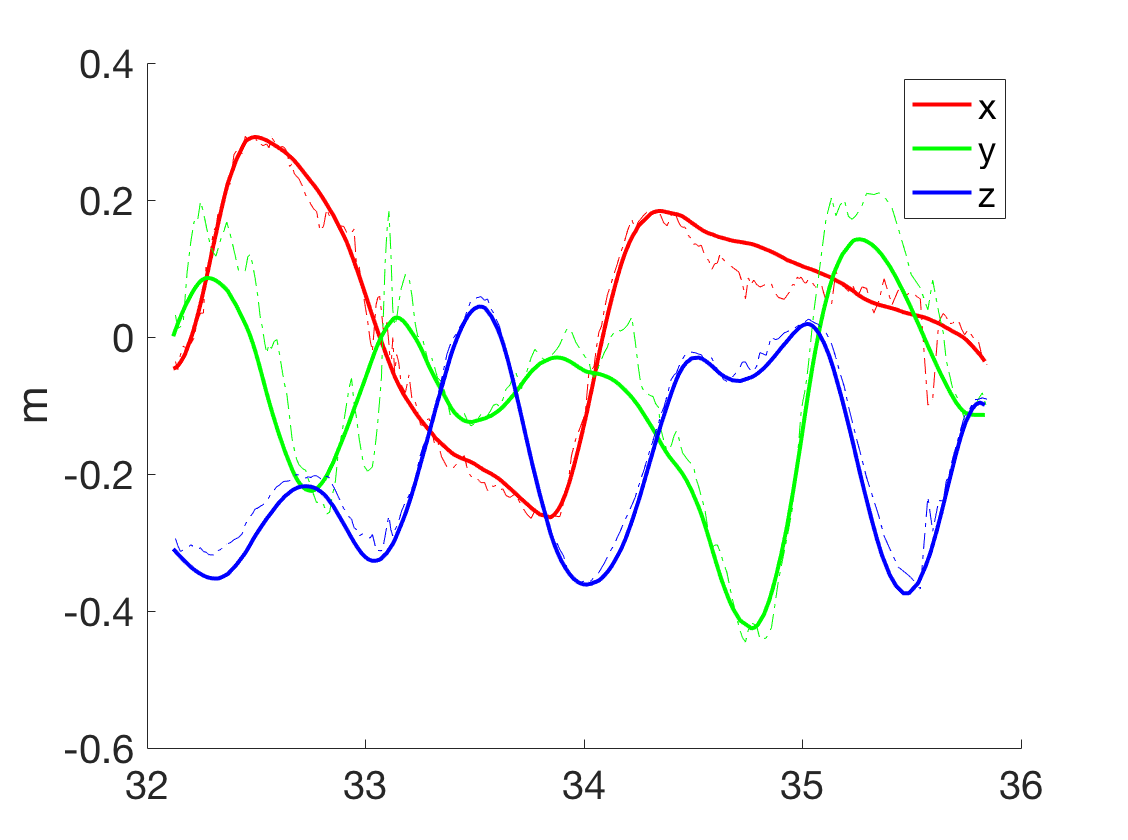
\includegraphics[width =
    \textwidth]{images/shapes_6dof_translation_33.png} (b) Translation
  \end{minipage}
  \hfill
  \caption{\textit{shapes\_6dof} sequence. Comparison of the estimated
    pose (dashed line) against ground truth (full line) within
    segments of 8 seconds duration.}
  \label{fig:shapes_6dof_pose_zoomed}
\end{figure}
A quantitative error estimation is included in \cref{tab:err_est}. The
window sizes for \textit{shapes} and \textit{poster} sequences are
4000 and 30000, respectively. Also, we used the \textit{Nelder-Mead Simplex}
algorithm provided by \textit{GNU-GSL}\citep{gough2009gnu}
to perform the optimization on \textit{shapes} sequences, and the
\textit{Fletcher-Reeves conjugate gradient}\citep{fletcher2013practical} algorithm to perform
optimization on the \textit{poster} dataset. Both methods work. The
analytic differentiation is faster and more stable. However, when the
initial guess is further from the ground truth, the numeric
differentiation seems to work better than the analytic
differentiation, since the jacobians used for analytic differentiation
are strictly local (see appendix). whereas a properly chosen step size
for numeric differentiation
\begin{itemize}
\item median\\
\item percent\\
\item scene depth no drift\\
\end{itemize}

\begin{table}[h]
  \label{tab:err_est}
  \begin{center}
    \begin{tabular}{lcccccl}
      \hline
      \multirow{3}{*}{Dataset}&\multicolumn{3}{c}{Median Orientation}&\multirowcell{3}{Median Translation \\ Error/m}&\multirowcell{3}{Traveled\\Distance}&\multirow{3}{*}{Note}\\
                              &\multicolumn{3}{c}{Error/deg}& &\\
      \cline{2-4}
                              & pitch&  yaw & roll &       &       &                  \\
      \hline
      shapes\_6dof        & 1.89 & 1.01 & 0.85 & 0.047 & 46.89 & Tracked all 60s  \\
      shapes\_translation & 0.85 & 0.45 & 0.27 & 0.019 & 14.08 & Lost after 25.0s \\
      poster\_6dof        & 1.14 & 1.22 & 0.63 & 0.054 & 12.50 & Lost after 22.8s \\
      poster\_translation & 0.55 & 0.57 & 0.25 & 0.022 & 11.14 & Lost after 26.0s \\
      \hline
    \end{tabular}
  \end{center}
  \caption{Quantitative evaluation on planar sequences}
\end{table}


% \begin{table}[h]
%   \label{tab:err_est}
%   \begin{center}
%     \begin{tabular}{lcccccccl}
%       \hline
%       &\multicolumn{3}{c}{Median Orientation}& \multicolumn{3}{c}{Median Translation}&Travelled Distance&Note \\
%       Dataset&\multicolumn{3}{c}{Error/deg}& \multicolumn{3}{c}{Error/m}&\\
%       \cline{2-9}
%       & pitch & yaw&roll&x&y&z&& \\
%       \hline
%       shapes\_6dof        & 1.47 & 2.94 &1.39 &0.019&0.036&0.014&46.89&med 0.0474     \\
%       shapes\_translation & 1.02 & 1.85 &0.31 &0.010 &0.021 &0.012&11.46&med 0.0292 \\
%       poster\_6dof& stuffed     & 92.50  &&0.027&0.018&0.035&12.5&med 0.054    lost after 22.8s    \\
%       poster\_translation& 0.55     & 0.57   &0.25&0.009&0.010&0.014&11.14&med 0.0221  lost after 26.03s \\
%       \hline
%     \end{tabular}
%   \end{center}
%   \caption{Quantitative evaluation on planar sequences}
% \end{table}


Despite of the rapid movements, in the above datasets the camera
actually only moves in a relative small region in front of the
textured plane, as depicted in \cref{fig:shapes_6dof_path}. However,
this method also applies when camera travels a longer distance with
respect to the scene depth, as shown in
\cref{fig:slider_hdr_far_map}. Also, although this method is designed
for planar scenes, in a complex scene with rotation only movement,
where no scene parameters are needed, this method can still be applied
to build a global map, delivering a result similar to \textit{image
  stitching}. \Cref{fig:boxes_rotation_map} is such an example.
\begin{figure}
  \centering
  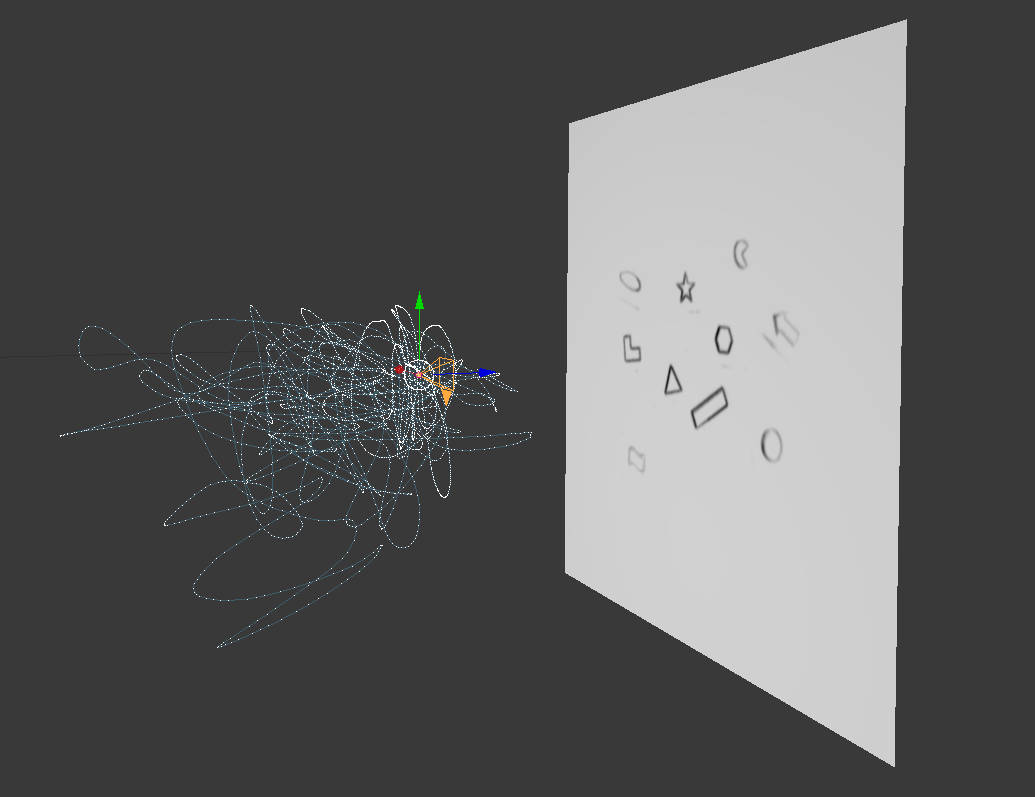
\includegraphics[width=\textwidth]{images/shapes_6dof_path.png}
  \caption{The motion path of the dataset
    \textit{shapes\_6dof}. Despite a trajectory length of about $50m$,
    in the whole $60s$ the camera actually stays in a relative small
    region compared to the scene depth, and there is no observable
    increase of drift using the method in this
    work. \textcolor{red}{ref to error estimation}}
  \label{fig:shapes_6dof_path}
\end{figure}
\begin{figure}
  \centering
  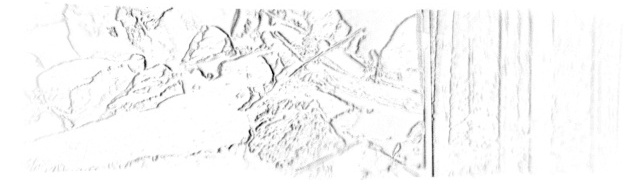
\includegraphics[width=\textwidth]{images/slider_hdr_far_map_36.jpg}
  \caption{The dataset \textit{slider\_hdr\_far}, with a scene depth
    of $0.584 m$, and a camera movement in the positive $x$ direction
    only. Note that this is a much wider map than what we have seen
    before. The figure shows the result at $4.8 sec$ within the whole
    range of $6.3 sec$; afterwards the algorithm is lost in the
    forest, where almost all the textures are vertical, causing severe
    local optima problem. If we constrain the motion estimation to
    translation only, it delivers a much better result.}

  \label{fig:slider_hdr_far_map}
\end{figure}
\begin{figure}
  \centering
  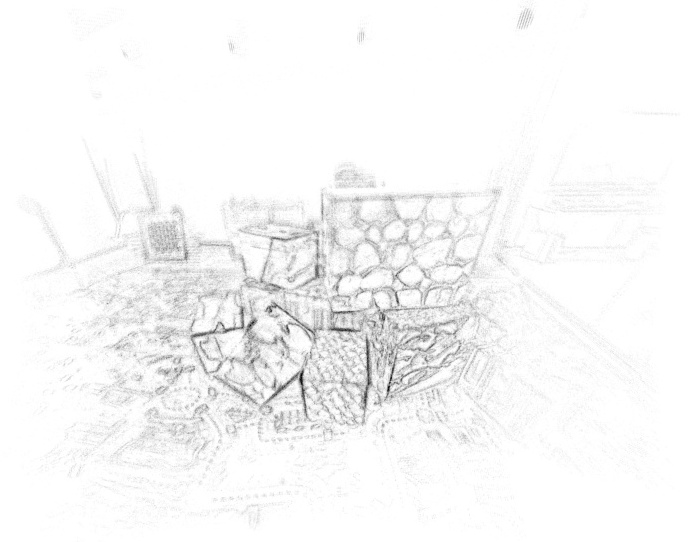
\includegraphics[width=\textwidth]{images/boxes_rotation_map.jpg}
  \caption{The dataset \textit{boxes\_rotation}. The motion in this
    dataset is rotation-dominated}
  \label{fig:boxes_rotation_map}
\end{figure}




\chapter{A Discussion to 6DoF Motion Estimation in General 3D Scenes}
\label{chap:general_scene}

For general 3D scenes with complex scene structure, we may consider
dividing the scene into multiple patches, and assume each patch is a
plane.

Without knowing which parts of the scene correspond to real planes in
space, we may simply divide the image into $4\times3$ regular grids,
assign each event to the grid it belongs with a different set of
parameters (2 for plane normal and 1 for depth), and optimize the
frame with one single motion model. Accounting for the scale
ambiguity, this amount to $(3\times12+5=)41$ parameters for each
\textit{per-frame} optimization. The scale ambiguity is solved by
parametrizing the linear velocity with 2 parameters
$(\phi,\psi)\in\mathbb{S}^2$ indicating its direction, the same as the
parametrization of a plane normal. This parametrization can not
describe zero velocity; however, for the hand-held datasets we tested
on this is not a problem. \textcolor{red}{normalize \& fix one depth
  value?} Note that we don't need to optimize each patch individually
and sum the costs together, since the intensity computation
\cref{eq:intensity} naturally sums all the events together so that we
only need one cost function for one image. Also, the regions with
fewer events have more pixels with zero intensity and thus have lower
contribution to the cost function \cref{eq:variance}, so no extra
weighting is needed.

In \cref{fig:patches_compr}, we compare the synthesized images before
and after motion correction of some selective images in various
sequences. After motion correction, the edges appear much sharper.

Since each frame has a different scale, without a global map as in
\cref{sec:frame2map}, it's hard to measure the accuracy of the linear
velocity estimation. We first give the estimation of angular velocity
in \cref{tab:err_est_planar}. Comparing line 1 with line 2, line 3 and
line 4, we can see that for general 3D scenes, planar patches
assumption delivers better result than assuming the whole scene as one
single plane. Notice that planar patches assumption for general scene
has a similar error magnitude as planar assumption for planar scenes
(line 6 and 8). However, the angular velocity estimated by either
planar or planar patches assumption can not achieve the accuracy when
estimating scenes with rotation dominated movements (line 5 and 7).

Without known scale for each frames, we can compare the angles between
ground truth and estimated linear velocities. It turns out that for
either planar scenes or planar patches assumption for general scenes,
the mean angle is around \unit[50]{\degree}, which is much larger than that
of angular velocity, which is around \unit[20]{\degree}. We guess that the
window size is not large enough to provide a sufficient baseline for
linear velocity estimation. But the window size can also not be chosen
too large, otherwise the constant velocity assumption would fail. We
already see in \cref{sec:planar_scenes} that the inaccuracy problem
can be solved by building a map and track on the map over a
distance. For general scenes -----

\begin{figure}
  \begin{minipage}[t]{0.48\textwidth}
    \centering 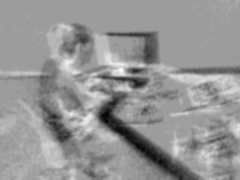
\includegraphics[width =
    \textwidth]{images/zero_motion_934.jpg} (a)
  \end{minipage}
  \hfill
  \begin{minipage}[t]{0.48\textwidth}
    \centering 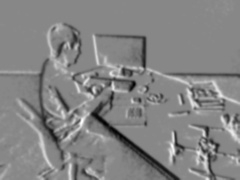
\includegraphics[width =
    \textwidth]{images/optimized_934.jpg} (b)
  \end{minipage}
  \hfill
  \begin{minipage}[t]{0.48\textwidth}
    \centering 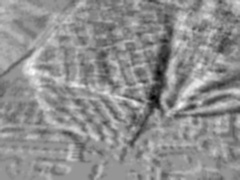
\includegraphics[width =
    \textwidth]{images/zero_motion_1321.jpg} (c)
  \end{minipage}
  \hfill
  \begin{minipage}[t]{0.48\textwidth}
    \centering 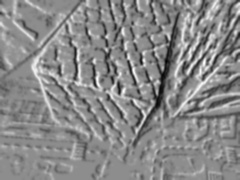
\includegraphics[width =
    \textwidth]{images/optimized_1321.jpg} (d)
  \end{minipage}
  \hfill
  \begin{minipage}[t]{0.48\textwidth}
    \centering 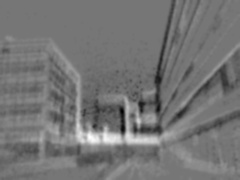
\includegraphics[width =
    \textwidth]{images/zero_motion_2390.jpg} (e)
  \end{minipage}
  \hfill
  \begin{minipage}[t]{0.48\textwidth}
    \centering 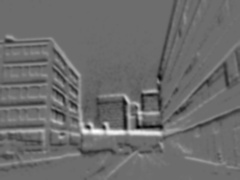
\includegraphics[width =
    \textwidth]{images/optimized_2390.jpg} (f)
  \end{minipage}
  \hfill
  \caption{Test results on 3 sequences with 6DoF
    motion. \textit{Left}: Accumulated events without motion
    compensation. \textit{Right:} Images after motion compensation via
    dividing scene into 12 regular grids. (a)(b)
    \textit{dynamic\_6dof} sequence, with ground truth velocities
    $\bm{\omega}=(-0.145;-3.761;1.925) \unitfrac{rad}{s},
    \vec{v}=(0.313;0.855;0.326) \unitfrac{m}{s}$. (c)(d) \textit{boxes\_6dof}
    sequence, with ground truth velocities
    $\bm{\omega}=(-1.357;0.981;4.577) \unitfrac{rad}{s},
    \vec{v}=(2.805;0.538;-0.676) \unitfrac{m}{s}$. (e)(f)
    \textit{outdoors\_running} sequence, with no ground truth
    information available.}
  \label{fig:patches_compr}
\end{figure}

\begin{figure}
\centering 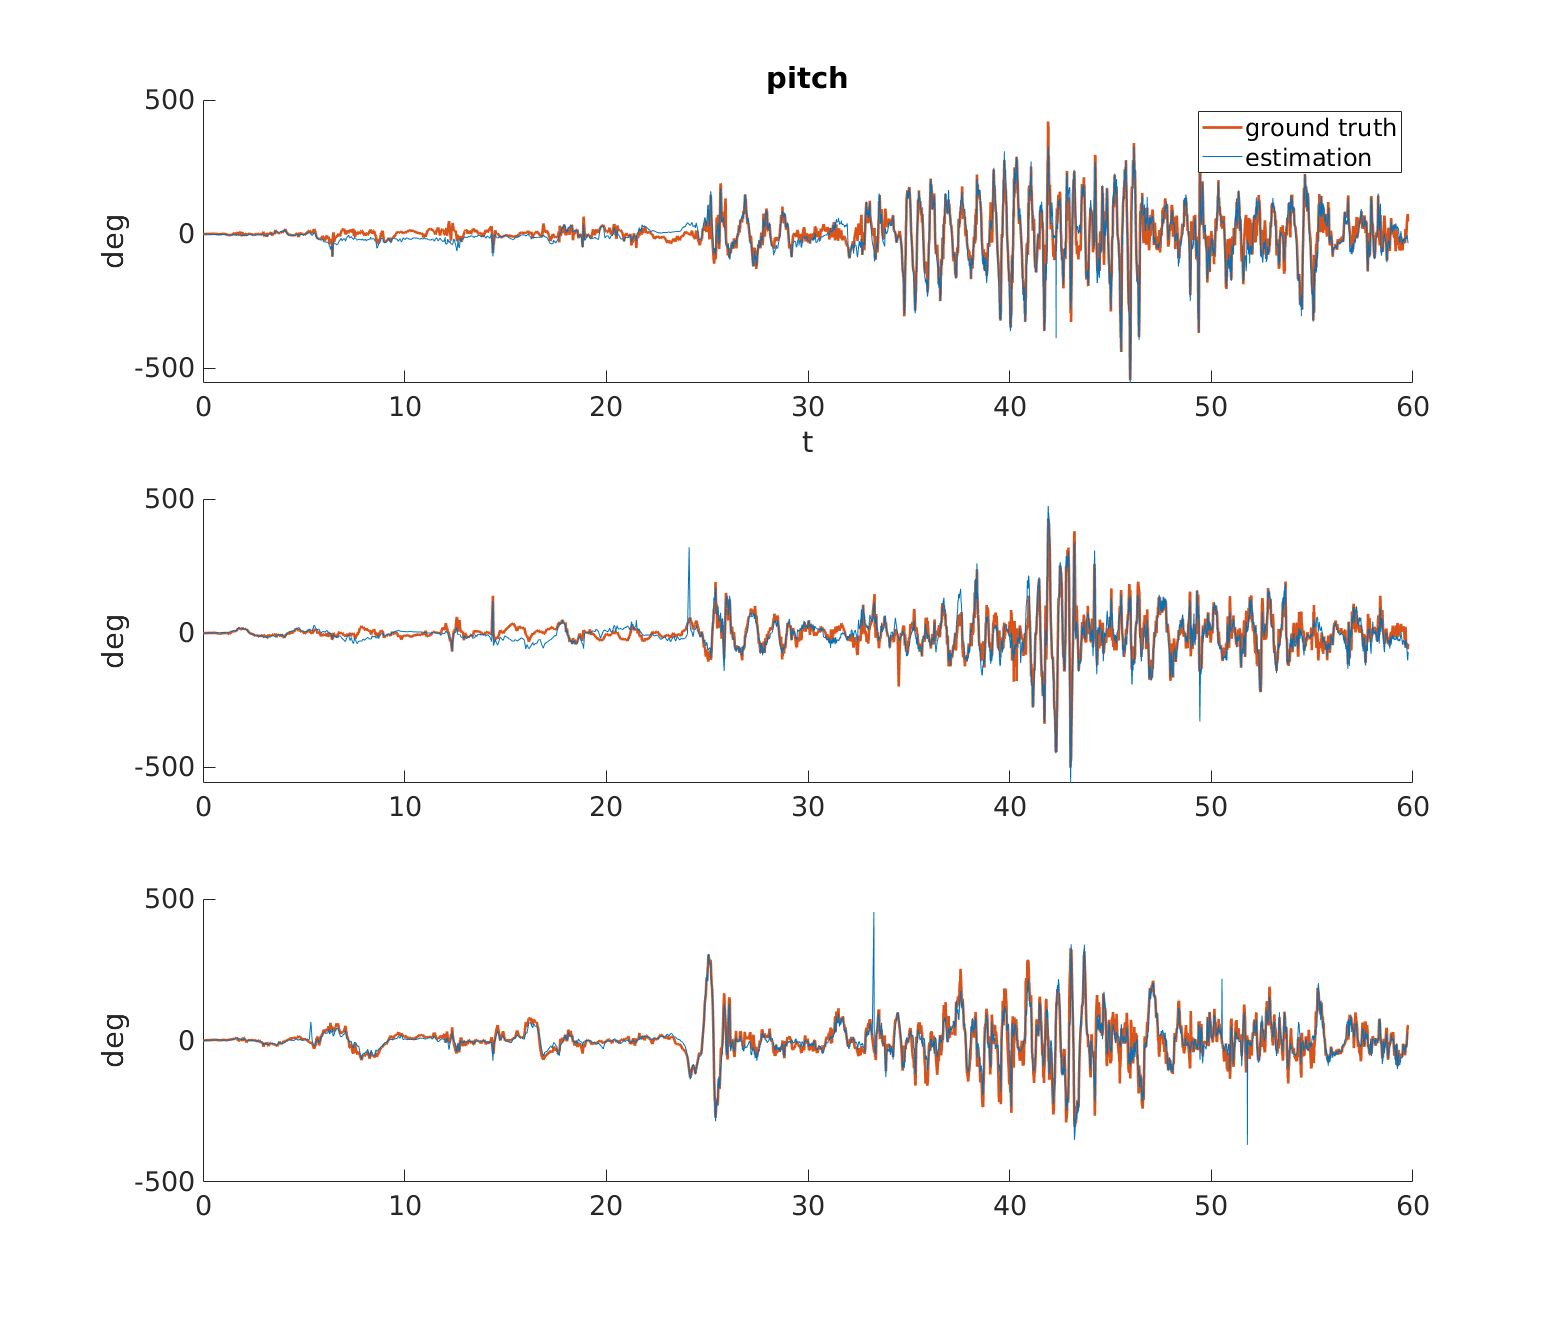
\includegraphics[width =
\textwidth]{images/boxes_6dof_rotation_.png}
\label{fig:boxes_6dof_rotation}
\caption{boxes 6dof rotation}
\end{figure}

\begin{table}[h]
  \label{tab:err_est_planar}
  \begin{center}
    \begin{tabular}{rlccccl}
      \hline
      \multirow{3}{*}{No.}&\multirow{3}{*}{Dataset}&\multicolumn{3}{c}{Median Orientation}&\multirowcell{3}{Maximal\\Velocity\\(\unitfrac{\degree}{s})}&\multirow{3}{*}{Parametrization}\\
                          &                     &\multicolumn{3}{c}{Error (\unit{\degree})}& &\\
      \cline{3-5}
                          &                    & pitch&  yaw & roll &          &                  \\
      \hline\hline
      1&dynamic\_6dof    & 20.88 & 21.60 & 18.08 & 509.37 & 6DoF, 12 patches \\
      2&boxes\_6dof      & 34.69 & 27.49 & 20.21 & 428.19 & 6DoF, 12 patches \\
      3&boxes\_6dof      & 60.16 & 31.33 & 21.11 & 428.19 & 6DoF, planar assumption \\
      4&boxes\_rotation  & 9.39 & 9.84 & 12.55 &679.78& 3DoF (angular velocity)\\
      5&poster\_6dof     & 32.23 & 31.55 & 22.37  & 905.58 & 6DoF, planar assumption\\
      6&poster\_rotation & 11.62 & 8.47  & 13.23  & 934.88 & 3DoF (angular velocity) \\
      7&poster\_rotation & 36.45 & 27.00 & 26.14 &905.58& 6DoF, planar assumption\\

      \hline
    \end{tabular}
  \end{center}
  \caption{Comparison between planar assumption, planar patches
    assumption and rotation only estimation. The maximal velocity
    computes the maximal velocities among all three axes}
\end{table}

\label{sec:note}

tried initialize with multiple frames, didn't work very
well. similarly sliding window didn't work; too many events didn't
work

\chapter{Conclusion and Outlook}
\label{chap:conclusion}

We found that the calibration matrix provided in
\citep{mueggler2017event} is not very accurate, edges close to the
upper left corner of the image always appear curved. We checked their
provided calibration dataset, and found that the checkerboard has
barely any corners in the upper left part of the image, which should
be the reason why the undistortion in that area is not working
well. This might be one of the causes why sometimes the image-to-model
matching is not performing well. We also tried to cropped part of the
image, but the resolution of DAVIS is relatively low (240$\times$180),
cropping reduces the amount of information and does not work better.

Usually the maps of \emph{shapes} and \emph{poster} sequences are done
after 6 and 10 keyframes, respectively; as the number of keyframes
increases, the size of the parameter set also increases (116
parameters in the bundle adjustment phase with 10 keyframes), which
makes the problem hard to optimize. For a least square optimizing
problem, which is often encountered in visual odometry, the
Levenberg-Marquardt algorithm\citep{press1988numerical} is a good
iteration method. However, the cost function \cref{eq:variance} used
in this work is a more general non-linear function, and thus harder to
optimize. The Nelder-Mead Simplex algorithm\citep{nelder1965simplex}
used in bundle adjustment phase is better suitable for problems with
small parameter size, and the choice of the initial simplex size is
important. In the per-frame optimization and frame-to-model matching
phase we make use of the derivatives; both BFGS and conjugate gradient
approximate the objective function by a quadratic hypersurface, thus
work well only when the evaluation point is close enough to the
optimum. For a more reliable tracking over a longer distance, we
should consider if better strategies are available, for example
optimize only a subset of the keyframes that are most important for
the current frame or most recent, or try multiple starting points.

DVS: 130 dB (~1 lux**); APS: 55 dB
